\begin{scope}
    
    \begin{scope}[yshift=\distancebetweenlayers,
        every node/.append style={yslant=-0.5,xslant=1},
        yslant=-0.5,xslant=1]
        \node[inner sep=0] (image1) {
            \phantom{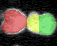
\includegraphics[width=\scalingfactor\textwidth]{images/joint/78_seg_crop.png}}
        };
        \begin{pgfonlayer}{upper}
            \begin{scope}[every node/.append style={scale=0.7}]
                \node[fg_det, label={[font=\tiny]center:$X_1^t$}] (a1) at (image1.south east) {};
                \node[fg_det, label={[font=\tiny]center:$X_2^t$}] (a2) at ($(image1.south east)!0.5!(image1.north east)$) {};
                \node[fg_det, label={[font=\tiny]center:$X_3^t$}] (a3) at (image1.north east) {};
                \node[fg_det, label={[font=\tiny]center:$X_5^t$}] (a5) at ($(image1.south west)!0.5!(image1.north west)$) {};
                \node[fg_det, label={[font=\tiny]center:$X_4^t$}] (a4) at ($(a3)!0.5!(a5)$) {};
            \end{scope}
            \begin{scope}[every node/.append style={scale=0.65}]
                \node[conflict,yshift=-5] (c1) at ($(a1)!0.5!(a5)$) {};
                \node[conflict, right=of a3, xshift=-10, yshift=-10] (c2) {};
                \node[conflict, yshift=-20] (c3) at (a4) {};
                \node[count, yshift=-20] (c4)  at ($(a2)!0.5!(a4)$) {};
                
                \path[count] (a1) edge (c4);
                \path[count] (a2) edge (c4);
                \path[count] (a3.south) edge (c4);
                \path[count] (a4) edge (c4);
                \path[count] (a5) edge[bend right=20] (c4);
                
                \path[conflict] (a5) edge[bend right=10] (c1);
                \path[conflict] (a1) edge (c1);

                \path[conflict] (a2) edge (c2);
                \path[conflict] (a4) edge[bend left=50] (c2);
                \path[conflict] (a5) edge[bend left=65] coordinate[pos=0.65](helpercoord1) (c2);

                \path[conflict] (a3) edge[bend left=10] (c3);
                \path[conflict] (a4) edge (c3);
                \path[conflict] (a5) edge (c3);
            \end{scope}
        \end{pgfonlayer}
        \begin{pgfonlayer}{bgupper}
            \node[rectangle, color=black,thick, fill=hypothesesbackground!30, opacity=0.8, draw=black,
            fit=(a1) (c2) (a5) (helpercoord1), inner sep=2, opacity=0.8, label={[xshift=15]above:{$t\phantom{+1}$}}]
            (bgup) {};
        \end{pgfonlayer}
    \end{scope}

    \begin{scope}[every node/.append style={yslant=-0.5,xslant=1},yslant=-0.5,xslant=1]
        \node[inner sep=0] (image2) {
            \phantom{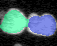
\includegraphics[width=\scalingfactor\textwidth]{images/joint/79_seg_crop.png}}
        };
        
        \begin{pgfonlayer}{bglower}
            \node[rectangle, color=black,thick, fill=hypothesesbackground!30, opacity=0.8, draw=black,
            fit=(a1) (c2) (a5) (helpercoord1), inner sep=2, opacity=0.8, shift=($(image2) - (image1)$), label={[xshift=15]above:{$t+1$}}]
            (bglow) {};
        \end{pgfonlayer}
        \begin{pgfonlayer}{lower}
            \begin{scope}[every node/.append style={scale=0.7}]
                \node[fg_det, label={[font=\tiny]center:$X_6^{t+1}$}] (b1) at (image2.south east) {};
                \node[fg_det, label={[font=\tiny]center:$X_7^{t+1}$}] (b2) at (image2.north east) {};
                \node[fg_det, label={[font=\tiny]center:$X_8^{t+1}$}] (b3) at ($(image2.south west)!0.5!(image2.north west)$) {};
            \end{scope}
            \begin{scope}[every node/.append style={scale=0.65}]
                \path[conflict] (b1) edge (b3);
                \path[conflict] (b3) edge (b2);
                \node[conflict, label=below left:$\psi_{\text{det}}$] (c1) at ($(b1)!0.5!(b3)$) {};
                \node[conflict] (c2) at ($(b2)!0.5!(b3)$) {};
                \node[count, label=right:$\psi_{\text{count}}$] (c3) at ($(b1)!0.5!(b2)!0.3!(b3)$) {};
                \path[count] (b1) edge (c3);
                \path[count] (b2) edge (c3);
                \path[count] (b3) edge (c3);
            \end{scope}
        \end{pgfonlayer}
    \end{scope}

    \begin{pgfonlayer}{transition}
        \begin{scope}[every node/.append style={scale=0.9}]
            \node[fg_tra,label={[font=\tiny]center:$Y_{1,6}^t$},xshift=0] (trans1) at ($(a1)!0.55!(b1)$) {};
        \end{scope}
        \begin{scope}[every node/.append style={scale=0.7}]
            \node[transfac, label=right:$\psi_{\text{out}}$] (out) at ($(a1.center)!0.5!(trans1)$) {};
            \node[transfac, label=right:$\psi_{\text{in}}$] (in) at ($(b1.center)!0.5!(trans1)$) {};
            \path[transfac] (a1) edge (out.center);
            \path[transfac] (out) edge (trans1);
            \path[transfac] (trans1) edge (in);
            \path[transfac] (in) edge (b1.center);
        \end{scope}
        \begin{scope}[every node/.append style={scale=0.9}]
            \node[fg_tra,label={[font=\tiny]center:$Y_{1,7}^t$},xshift=0,yshift=0] (trans2) at ($(out)!0.35!(b2)$) {};
        \end{scope}
        \begin{scope}[every node/.append style={scale=0.7}]
            \node[transfac] (in2) at ($(b2.center)!0.5!(trans2)$) {};
            \path[transfac] (out) edge (trans2);
            \path[transfac] (trans2) edge (in2);
            \path[transfac] (in2) edge (b2.center);
        \end{scope}
    \end{pgfonlayer}
    \coordinate (base1) at (bglow.north west |- bglow.south west);
    \coordinate (base2) at (bglow.south east |- bglow.south west);
    % \draw [pllbl] (base1) -- (base2) node[black,midway,yshift=-0.6cm] {Factor Graph};
    % \path let \p1 = (base1.west), \p2 = (base2.east) in
    % node[pllbltxt, minimum width=\x2-\x1] (labelgraph) at ($(base1)!0.5!(base2)$) {Factor Graph};
\end{scope}


%%% Local Variables: 
%%% mode: latex
%%% TeX-master: "../../main"
%%% End: 
